\section{Use case}
\label{sec:use_case}
Gli \textit{use case} sono uno strumento grafico che permette di analizzare e approfondire i requisiti utente per arrivare a definire i requisiti software del sistema.

\subsection{Descrizione Use Case}

\begin{figure}[H]
    \centering
    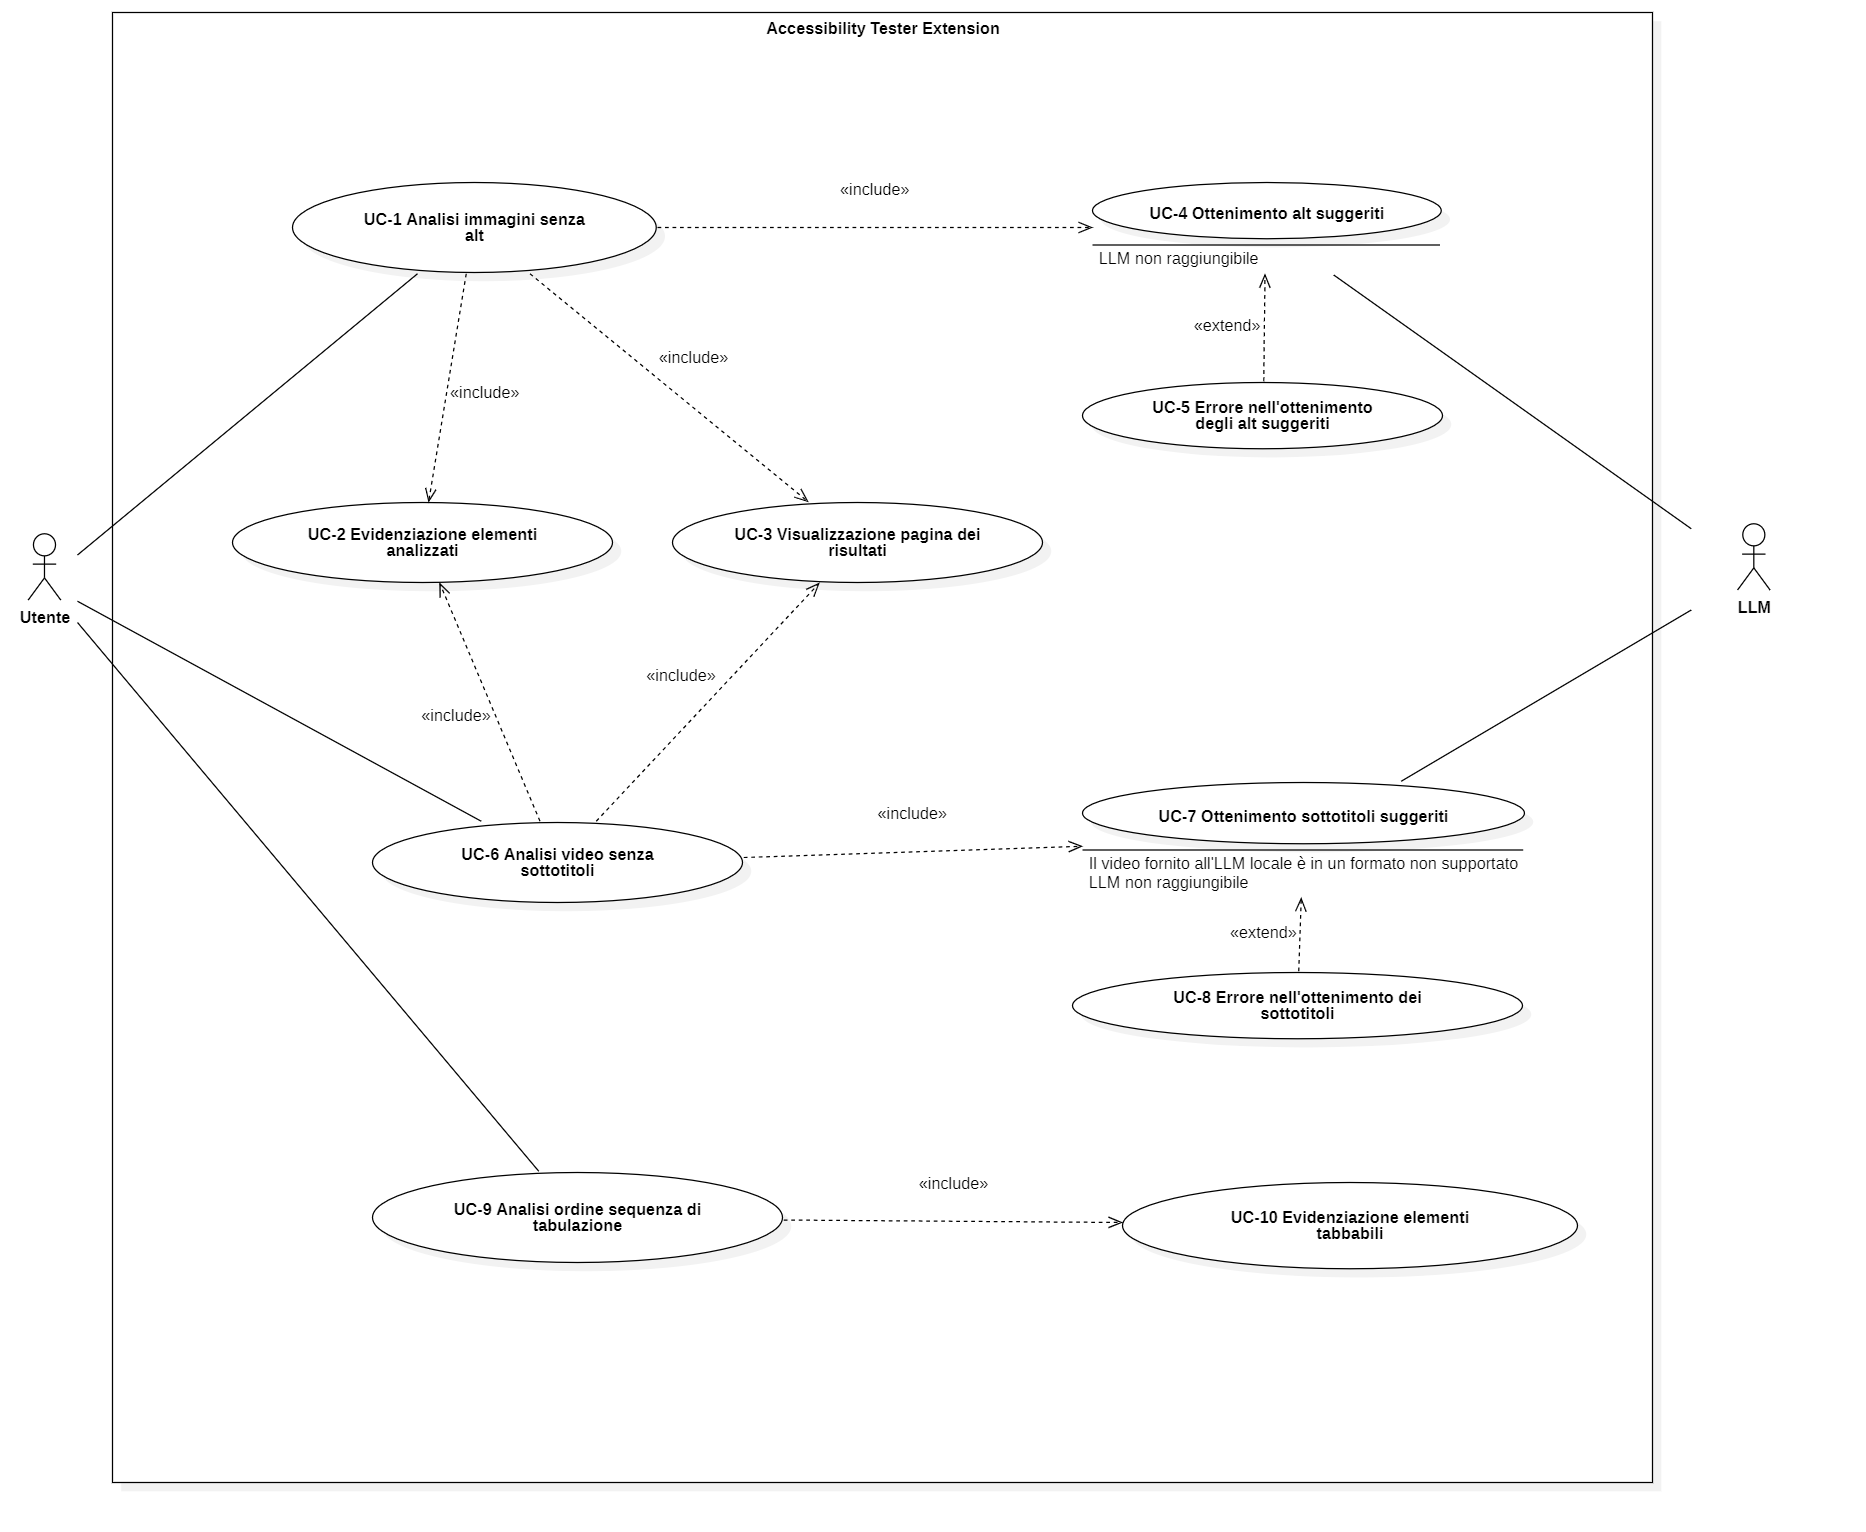
\includegraphics[width=\linewidth]{Sezioni/UseCase/Immagini/Generale.png}
    \caption{Diagramma generale use case}
\end{figure}

\begin{usecase}{UC-1}{Analisi immagini senza alt} 
    \label{uc:UC-1}

    \pre{} 
    
    \post{
        \item Vengono visualizzate le immagini analizzate
    }

    \actor{Utente} 

    \trigger{L'utente ha premuto sul pulsante per iniziare l'analisi delle immagini} 

    \inc{\hyperref[uc:UC-2]{UC-2}, \hyperref[uc:UC-3]{UC-3}, \hyperref[uc:UC-4]{UC-4}}

    \base{} 

    \scenario{ 
        \item L'utente preme il pulsante per avviare l'analisi delle immagini
                    
        \item Il sistema verifica la presenza nella pagina di immagini senza alt
             
        \item Il sistema evidenzia le immagini senza alt seguendo \hyperref[uc:UC-2]{UC-2}

        \item Il sistema ottiene suggerimenti per gli alt delle immagini seguendo \hyperref[uc:UC-4]{UC-4}
        
        \item Il sistema mostra un messaggio che indica l'assenza di immagini senza alt oppure mostra le immagini individuate seguendo \hyperref[uc:UC-3]{UC-3}
    } 

    \subscenario{} 
  \end{usecase}
  
  \begin{usecase}{UC-2}{Evidenziazione elementi analizzati} 
    \label{uc:UC-2}

    \pre{
        \item Il sistema ha rilevato delle immagini senza alt o dei video senza sottotitoli
    } 
    
    \post{
        \item Gli elementi rilevati vengono evidenziati con un bordo rosso
    }

    \actor{Utente} 

    \trigger{L'analisi rileva almeno un elemento} 

    \inc{}

    \base{} 

    \scenario{
        \item Il sistema aggiunge un bordo rosso ad ogni elemento rilevato dall'analisi
    } 

    \subscenario{} 
  \end{usecase}

  \begin{usecase}{UC-3}{Visualizzazione pagina dei risultati} 
    \label{uc:UC-3}

    \pre{
        \item Il sistema ha terminato l'analisi delle immagini senza alt o dei video senza sottotitoli
    } 
    
    \post{
        \item L'utente visualizza un sottogruppo degli elementi analizzati
    }

    \actor{Utente} 

    \trigger{Il sistema deve mostrare gli elementi analizzati all'utente} 

    \inc{}

    \base{} 

    \scenario{
        \item Il sistema termina l'analisi degli elementi
        \item Il sistema ha rilevato immagini senza alt o video senza sottotitoli
        \item Il sistema mostra, a gruppi, gli elementi rilevati dall'analisi
    } 

    \subscenario{} 
  \end{usecase}

  \begin{usecase}{UC-4}{Ottenimento alt suggeriti} 
    \label{uc:UC-4}

    \pre{
        \item Il sistema ha rilevato la presenza di immagini senza alt
    } 
    
    \post{
        \item Per ogni immagine senza alt individuata, il sistema ottiene il relativo suggerimento di testo alternativo
    }

    \actor{Utente} 

    \subactors{LLM}

    \trigger{Il sistema deve ottenere dei suggerimenti per i testi alternativi delle immagini} 

    \inc{}

    \base{} 

    \scenario{
        \item Il sistema effettua, per ogni immagine rilevata, una richiesta all'LLM
        \item Il sistema ottiene, per ogni immagine rilevata, un testo alternativo per l'immagine come suggerimento
    } 

    \subscenario{
        \item[1.1] Errore interno durante il collegamento con l'LLM
        \begin{itemize}
            \item \hyperref[uc:UC-5]{UC-5}
        \end{itemize}
    } 
  \end{usecase}

  \begin{usecase}{UC-5}{Visualizzazione errore nell'ottenimento degli alt suggeriti} 
    \label{uc:UC-5}

    \pre{
        \item Avviene un errore interno al sistema durante la richiesta all'LLM
    } 
    
    \post{
        \item L'utente è a conoscenza dell'errore avvenuto
    }

    \actor{Utente} 

    \trigger{Il sistema ha provato a comunicare con l'LLM per ottenere un alt suggerito} 

    \inc{}

    \base{} 

    \scenario{
        \item Il sistema notifica all'utente, mediante un messaggio di errore, la causa dell'anomalia
    } 

    \subscenario{} 
  \end{usecase}

  \begin{usecase}{UC-6}{Analisi video senza sottotitoli} 
    \label{uc:UC-6}

    \pre{} 
    
    \post{
        \item Vengono visualizzati i video analizzati
    }

    \actor{Utente} 

    \trigger{L'utente ha premuto sul pulsante per iniziare l'analisi dei video} 

    \inc{\hyperref[uc:UC-2]{UC-2}, \hyperref[uc:UC-3]{UC-3}, \hyperref[uc:UC-7]{UC-7}}

    \base{} 

    \scenario{ 
        \item L'utente preme il pulsante per avviare l'analisi dei video
                    
        \item Il sistema verifica la presenza nella pagina di video senza sottotitoli
             
        \item Il sistema evidenzia i video senza sottotitoli seguendo \hyperref[uc:UC-2]{UC-2}

        \item Il sistema ottiene suggerimenti per i sottotitoli dei video seguendo \hyperref[uc:UC-7]{UC-7}
        
        \item Il sistema mostra un messaggio che indica l'assenza di video senza sottotitoli oppure mostra i video individuati seguendo \hyperref[uc:UC-3]{UC-3}
    } 

    \subscenario{} 
  \end{usecase}

  \begin{usecase}{UC-7}{Ottenimento sottotitoli suggeriti} 
    \label{uc:UC-7}

    \pre{
        \item Il sistema ha rilevato la presenza di video senza sottotitoli
    } 
    
    \post{
        \item Per ogni video senza sottotitoli individuato, il sistema ottiene il relativo suggerimento di sottotitoli
    }

    \actor{Utente} 

    \subactors{LLM}

    \trigger{Il sistema deve ottenere dei suggerimenti per i sottotitoli dei video} 

    \inc{}

    \base{} 

    \scenario{
        \item Il sistema effettua, per ogni video rilevato, una richiesta all'LLM
        \item Il sistema ottiene, per ogni video rilevato, i sottotitoli per il video come suggerimento
    } 

    \subscenario{
        \item[1.1] Errore interno durante la comunicazione con l'LLM
        \begin{itemize}
            \item \hyperref[uc:UC-8]{UC-8}
        \end{itemize}
    } 
  \end{usecase}


  \begin{usecase}{UC-8}{Visualizzazione errore nell'ottenimento dei sottotitoli suggeriti} 
    \label{uc:UC-8}

    \pre{
        \item Avviene un errore interno al sistema durante la richiesta all'LLM
    } 
    
    \post{
        \item L'utente è a conoscenza dell'errore avvenuto
    }

    \actor{Utente} 

    \trigger{Il sistema ha provato a comunicare con l'LLM per ottenere dei sottotitoli suggeriti} 

    \inc{}

    \base{} 

    \scenario{
        \item Il sistema notifica all'utente, mediante un messaggio di errore, la causa dell'anomalia
    } 

    \subscenario{} 
  \end{usecase}

  \begin{usecase}{UC-9}{Analisi ordine sequenza di tabulazione} 
    \label{uc:UC-9}

    \pre{} 
    
    \post{
        \item Viene visualizzata una lista di anomalie nell'ordine della sequenza di tabulazione
    }

    \actor{Utente} 

    \trigger{L'utente ha premuto il pulsante per iniziare l'analisi dell'ordine della sequenza di tabulazione} 

    \inc{\hyperref[uc:UC-10]{UC-10}}

    \base{} 

    \scenario{
        \item L'utente preme il pulsante per avviare l'analisi dell'ordine della sequenza di tabulazione
        \item Il sistema ottiene tutti gli elementi tabbabili all'interno della pagina
        \item Il sistema evidenzia gli elementi tabbabili seguendo \hyperref[uc:UC-10]{UC-10}
        \item Il sistema verifica che gli elementi tabbabili all'interno di un contenitore semantico siano consecutivi
        \item Il sistema verifica che lo spostamento del tab tra due elementi consecutivi non vada dal basso verso l'alto o da destra verso sinistra
        \item Il sistema mostra un messaggio che indica l'assenza di anomalie nell'ordine della sequenza di tabulazione oppure indica le anomalie rilevate
    } 

    \subscenario{} 
  \end{usecase}

  \begin{usecase}{UC-10}{Evidenziazione elementi tabbabili} 
  \label{uc:UC-10}

    \pre{
        \item Il sistema ha rilevato elementi nella pagina con attributo tabindex assegnato
    } 
    
    \post{
        \item Vengono evidenziati gli elementi rilevati colorandone i bordi
    }

    \actor{Utente} 

    \trigger{L'analisi dell'ordine della squenza di tabulazione ha rilevato almeno un elemento con tabindex assegnato} 

    \inc{}

    \base{} 

    \scenario{
        \item Il sistema aggiunge un bordo rosso ad ogni elemento con tabindex positivo
        \item Il sistema aggiunge un bordo arancione ad ogni elemento con tabindex negativo
        \item Il sistema aggiunge un bordo verde ad ogni elemento con tabindex uguale a zero
    } 

    \subscenario{} 
  \end{usecase}

  

